
\item  The probes of a non-isolated, two-channel oscilloscope are clipped to points A, B and C in the circuit of the adjacent figure. $V_{\text{in}}$ is a square wave of a suitable low frequency. 
The display on Ch$_1$ and Ch$_2$ are as shown on the right. Then the ``Signal'' and ``Ground'' probes $S_1, G_1$ and $S_2, G_2$ of Ch$_1$ and Ch$_2$ respectively are connected to points:\hfill{(EE 2007)} 

\begin{figure}[H]
    \centering
    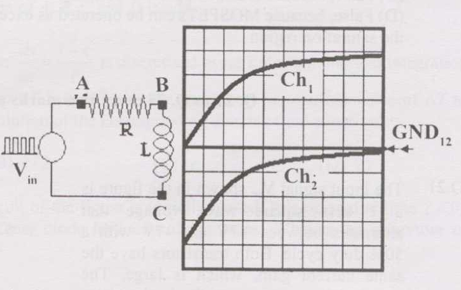
\includegraphics[width=0.6\linewidth]{figs/Q 17.png} \caption{}     \label{fig:myfigure}
   
\end{figure}

\begin{multicols}{4}
\begin{enumerate}
 \item  A,B,C,A
\item A,B,C,B
\item  C,B,A,B 
\item  B,A,B,C
\end{enumerate}
\end{multicols}

\item  The differential equation $\frac{dx}{dy}$ = $\frac{1-x}{\tau}$ is discretised using Euler's numerical integration method with a time step triangle $\Delta$T $>$  0 . What is the maximum permissible value of $\Delta$T to ensure stability of the solution of the corresponding discrete time equation?\hfill{(EE 2007)} 
\begin{multicols}{4}
\begin{enumerate}
 \item 1
\item $\frac{\tau}{2}$
\item $\tau$
\item 2$\tau$
\end{enumerate}
\end{multicols}
\item  \quad If $x = \text{Re}\ G(j\omega)$, and $y = \text{Im}\ G(j\omega)$ then for $\omega \to 0^{+}$, the Nyquist plot for\\
$G(s) = \dfrac{1}{s(s+1)(s+2)}$ becomes asymptotic to the line\hfill{(EE 2007)} 

\begin{multicols}{4}
\begin{enumerate}
\item  $x = 0$
\item  $x = -3/4$
\item  $x = y - 1/6$
\item  $x = y/\sqrt{3}$
\end{enumerate}
\end{multicols}


\vfill
\centering{EE 13/32}
\newpage

\item  \quad The system $\dfrac{900}{s(s+1)(s+9)}$ is to be compensated such that its gain-crossover frequency becomes same as its uncompensated phase-crossover frequency and provides a $45^{0}$ phase margin. To achieve this, one may use\hfill{(EE 2007)} 

\begin{enumerate}
    \item a lag compensator that provides an attenuation of 20 dB and a phase lag of $45^{0}$ at the frequency of $3\sqrt{3}$ rad/s
    \item a lead compensator that provides an amplification of 20 dB and a phase lead of $45^{0}$ at the frequency of 3 rad/s
    \item a lag-lead compensator that provides an amplification of 20 dB and a phase lag of $45^{0}$ at the frequency of $\sqrt{3}$ rad/s
    \item a lag-lead compensator that provides an attenuation of 20 dB and phase lead of $45^{0}$ at the frequency of 3 rad/s
\end{enumerate}

\item  \quad Consider the discrete-time system shown in the figure where the impulse response $G(z)$ is $g(0) = 0$, $g(1) = g(2) = 1$, $g(3) = g(4) = \cdots = 0$. \hfill{(EE 2007)} 

\begin{figure}[H]
    \centering
    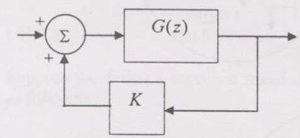
\includegraphics[width=0.4\linewidth]{figs/q 36 2007.png} 
\caption{}
    \label{fig:myfigure}
\end{figure}

This system is stable for range of values of $K$

\begin{multicols}{4}
\begin{enumerate}
\item  $[-1, 1/2]$
\item  $[-1, 1]$=
\item  $[-1/2, 1]$
\item  $[-1/2, 2]$
\end{enumerate}
\end{multicols}

\item A signal $x(t)$ is given by
$
x(t) = \begin{cases} 
1, & -\dfrac{T}{4} < t \leq \dfrac{3T}{4} \\\\ 
-1, & \dfrac{3T}{4} < t \leq \dfrac{7T}{4} \\\\ 
-x(t+T)
\end{cases}
$

Which among the following gives the fundamental Fourier term of $x(t)$?\hfill{(EE 2007)} 

\begin{multicols}{2}
\begin{enumerate}

\item  $\dfrac{4}{\pi} \cos\left(\dfrac{\pi t}{T} - \dfrac{\pi}{4}\right)$

\item  $\dfrac{\pi}{4} \cos\left(\dfrac{\pi t}{2T} + \dfrac{\pi}{4}\right)$

\item  $\dfrac{4}{\pi} \sin\left(\dfrac{\pi t}{T} - \dfrac{\pi}{4}\right)$

\item  $\dfrac{\pi}{4} \sin\left(\dfrac{\pi t}{2T} + \dfrac{\pi}{4}\right)$
\end{enumerate}
\end{multicols}



\item  If the loop gain $K$ of a negative feedback system having a loop transfer function $\dfrac{K(s+3)}{(s+8)^2}$ is to be adjusted to induce a sustained oscillation then\hfill{(EE 2007)} 

\begin{enumerate}
    \item The frequency of this oscillation must be $\dfrac{4}{\sqrt{3}}$ rad/s
    \item The frequency of this oscillation must be 4 rad/s
    \item The frequency of this oscillation must be 4 or $\dfrac{4}{\sqrt{3}}$ rad/s
    \item such a $K$ does not exist
\end{enumerate}
\centering{EE 14/32}
\newpage
\item   The system shown in figure below\hfill{(EE 2007)} 

\begin{figure}[H]
    \centering
    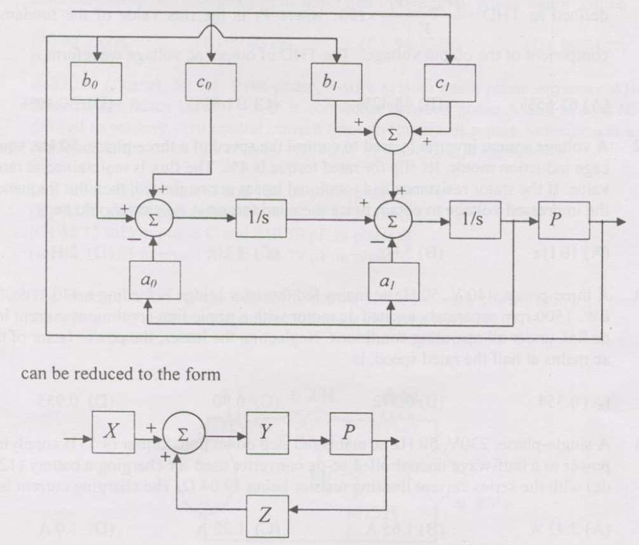
\includegraphics[width=0.75\linewidth]{figs/Q 39 2007.png} 
    \caption{}
    \label{fig:myfigure}
\end{figure}

with

\begin{enumerate}
   \item $X = c_0 s + c_1,$ \quad $Y = \dfrac{1}{s^{2} + a_0 s + a_1},$\quad $Z = b_0 s + b_1$

\item $X = 1,$ \quad $Y = \dfrac{c_0 s + c_1}{s^2 + a_0 s + a_1},$\quad $Z = b_0 s + b_1$

\item $X = c_1 s + c_0,$ \quad $Y = \dfrac{b_1 s + b_0}{s^2 + a_1 s + a_0},$\quad $Z = 1$

\item $X = c_1 s + c_0,$ \quad $Y = \dfrac{1}{s^2 + a_1 s + a_0},$\quad $Z = b_1 s + b_0$
\end{enumerate}
\item \quad A single-phase voltage source inverter is controlled in a single pulse-width modulated mode with a pulse width of $150^{\circ}$ in each half cycle. Total harmonic distortion is defined as $\text{THD} = \frac{\sqrt{V_{rms}^2 - V_1^2}}{V_1} \times 100$, where $V_1$ is the rms value of the fundamental component of the output voltage. The THD of output ac voltage waveform is\hfill{(EE 2007)} 

\begin{multicols}{4}
\begin{enumerate}
    \item  65.65\%
 \item  48.42\%
 \item 31.83\%
 \item  30.49\%
\end{enumerate}
\end{multicols}

\item The state equation for the current $I_1$ shown in the network shown below in terms of the voltage $V_x$ and the independent source $V$, is given by\hfill{(EE 2007)} 
\begin{figure}[H]
    \centering
    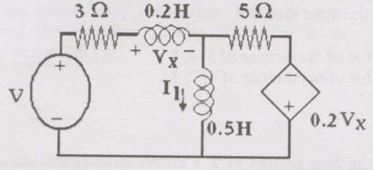
\includegraphics[width=0.45\linewidth]{figs/Q 50 2007.png} \caption{}     \label{fig:myfigure}
\end{figure}
\begin{enumerate}
   \item   $\dfrac{dI_1}{dt} = -1.4 V_x - 3.75 I_1 + \dfrac{5}{4} V$ 
\item  $\dfrac{dI_1}{dt} = 1.4 V_x - 3.75 I_1 - \dfrac{5}{4} V$
\item $\dfrac{dI_1}{dt} = -1.4 V_x + 3.75 I_1 + \dfrac{5}{4} V$
\item $\dfrac{dI_1}{dt} = -1.4 V_x + 3.75 I_1 - \dfrac{5}{4} V$

\end{enumerate}


\item \quad If $u(t)$, $r(t)$ denote the unit step and unit ramp functions respectively and $u(t)*r(t)$ their convolution, then the function $u(t+1)*r(t-2)$ is given by\hfill{(EE 2007)} 

\begin{multicols}{4}
\begin{enumerate} 
\item (1/2)$(t-1)(t-2)$
\item (1/2)$(t-1)(t-2)$
\item (1/2)$(t-1)^2u(t-1)$
\item none of the above
\end{enumerate}
\end{multicols}

\item The integral
$
\frac{1}{2\pi}\int_0^{2\pi}\sin(t-\tau)\cos\tau\, d\tau
$
equals\hfill{(EE 2007)} 

\begin{multicols}{4}
\begin{enumerate}
    \item $\sin t \cos t$
\item  $0$
\item  $(1/2) \cos t$
\item  $(1/2) \sin t$
\end{enumerate}
\end{multicols}

\vfill
\centering{EE 17/32}
\newpage


\item  \quad $X(z) = 1 - 3z^{-1}$,\quad $Y(z) = 1 + 2z^{-2}$ are Z-transforms of two signals $x[n],\,y[n]$ respectively.
A linear time invariant system has the impulse response $h[n]$ defined by these two signals as
$
    h[n] = x[n-1] * y[n]
$
where $*$ denotes discrete time convolution. Then the output of the system for the input $\delta[n-1]$\hfill{(EE 2007)} 
\begin{enumerate}
    \item has Z-transform $z^{-1} X(z) Y(z)$
    \item equals $\delta[n-2] - 3\delta[n-3] + 2\delta[n-4] - 6\delta[n-5]$
    \item has Z-transform $1 - 3z^{-1} + 2z^{-2} - 6z^{-3}$
    \item does not satisfy any of the above three.
\end{enumerate}


\item  \quad A loaded dice has following probability distribution of occurrences

\begin{center}
\begin{tabular}{|c|c|c|c|c|c|c|}
\hline
Dice value      & 1   & 2   & 3   & 4   & 5   & 6   \\
\hline
Probability     & $1/4$ & $1/8$ & $1/8$ & $1/8$ & $1/8$ & $1/4$ \\
\hline
\end{tabular}
\end{center}

If three identical dice as the above are thrown, the probability of occurrence of values 1, 5 and 6 on the three dice is\hfill{(EE 2007)} 
 
\begin{enumerate}
    \item same as that of occurrence of 3, 4, 5
    \item same as that of occurrence of 1, 2, 5
    \item$1/128$
    \item $5/8$
\end{enumerate}
\item  In the circuit shown in figure, switch SW$_1$ is initially CLOSED and SW$_2$ is OPEN. The inductor $L$ carries a current of $10~\mathrm{A}$ and the capacitor is charged to $10~\mathrm{V}$ with polarities as indicated. SW$_2$ is initially CLOSED at $t = 0-$ and SW$_1$ is OPENED at $t = 0$. The current through $C$ and the voltage across $L$ at $t = 0+$ is\hfill{(EE 2007)} 

\begin{figure}[H]
    \centering
    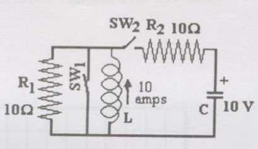
\includegraphics[width=0.3\linewidth]{figs/Q 61.png} \caption{}     \label{fig:myfigure}
\end{figure}


\begin{multicols}{4}
\begin{enumerate}
\item $55$A, $4.5$V
\item $5.5$A, $45$V
\item  $45$A, $5.5$V
\item $4.5$A, $55$V
\end{enumerate}
\end{multicols}

\vfill
\centering{EE 20/32}
\newpage
\item  \quad The R-L-C series circuit shown is supplied from a variable frequency voltage source. The admittance-locus of the R-L-C network at terminals AB for increasing frequency $\omega$ is\hfill{(EE 2007)} 

\begin{figure}[H]
    \centering
    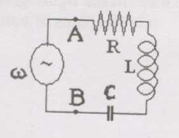
\includegraphics[width=0.3\linewidth]{figs/Q 62 Q.png} \caption{}     \label{fig:myfigure}
\end{figure}
    \begin{figure}[H]
    \centering
    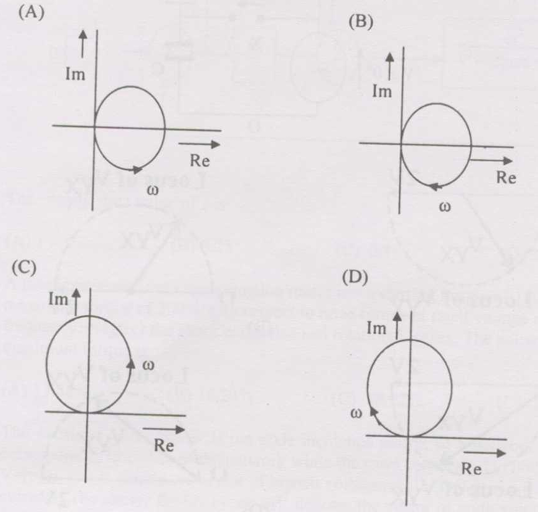
\includegraphics[width=0.85\linewidth]{figs/Q 62.png} 

\end{figure}
\vfill
\centering{EE 21/32}
\newpage
\item \quad In the figure given below all phasors are with reference to the potential at point ``O''. The locus of voltage phasor $V_{YX}$ as R is varied from zero to infinity is shown by\hfill{(EE 2007)} 

\begin{figure}[H]
    \centering
    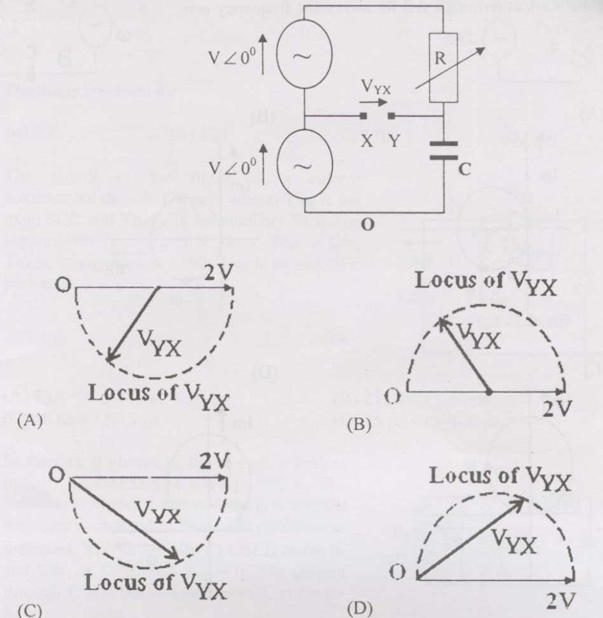
\includegraphics[width=1\linewidth]{figs/Q 63.png} \caption{}     \label{fig:myfigure}
\end{figure}
\vspace{1cm}
\item  \quad A 3V dc supply with an internal resistance of $2~\Omega$ supplies a passive non-linear resistance characterized by the relation $V_{NL} = I_{NL}^2$. The power dissipated in the non-linear resistance is\hfill{(EE 2007)} 

\begin{multicols}{4}
\begin{enumerate}
    \item $1.0$  
\item $1.5$ 
\item $2.5$ 
\item $3.0$ 
\end{enumerate}
\end{multicols}

\vfill
\centering{EE 22/32}
\newpage

\item  \hspace{0.5em} \parbox[t]{0.85\textwidth}{%
Consider the feedback control system shown below which is subjected to a unit step input. The system is stable and has the following parameters $k_p = 4$, $k_i = 10$, $\omega = 500$ and $\xi = 0.7$.
} 

\begin{figure}[H]
    \centering
    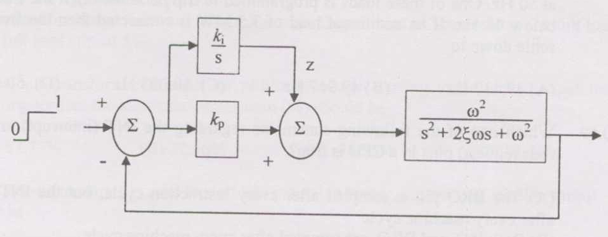
\includegraphics[width=0.7\linewidth]{figs/Q 65.png} \caption{}     \label{fig:myfigure}
\end{figure}

The steady state value of  is\hfill{(EE 2007)}
\begin{multicols}{4}
\begin{enumerate}
\item $1$  
\item $0.25$  
\item $0.1$  
\item $0$  
 \end{enumerate}
\end{multicols}

\textbf{Statement for Linked Answer Questions 80 \& 81:}\\
Consider the R-L-C circuit shown in figure.
\begin{figure}[H]
    \centering
    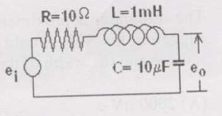
\includegraphics[width=0.3\linewidth]{figs/Q 80,81.png} \caption{}     \label{fig:myfigure}
\end{figure}
\item  For a step-input $e_i$, the overshoot in the output $e_o$ will be\hfill{(EE 2007)}

\begin{multicols}{4}
\begin{enumerate}
    \item  0, since the system is not under-damped
  \item 5\% 
  \item  16\% 
  \item  48\% 
\end{enumerate}
\end{multicols}

\item  If the above step response is to be observed on a non-storage CRO, then it would be best to have the $e_i$ as a\hfill{(EE 2007)}

\begin{multicols}{2}
\begin{enumerate}
 \item  step function 
\item square wave of frequency 50 Hz 
\item  square wave of frequency 300 Hz 
\item  square wave of frequency 2.0 kHz
\end{enumerate}
\end{multicols}
\newpage
\noindent
\textbf{Statement for Linked Answer Questions 82 \& 83:}\\
The associated figure shows the two types of rotate right instructions R1, R2 available in a microprocessor where Reg is a 8-bit register and C is the carry bit. The rotate left instructions L1 and L2 are similar except that C now links the most significant bit of Reg instead of the least significant one.

\vspace{0.5em}

\begin{figure}[H]
    \centering
    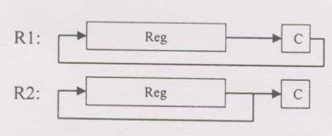
\includegraphics[width=0.5\linewidth]{figs/Q 82,83.png} \caption{}     \label{fig:myfigure}
\end{figure}

\textbf{Statement for Linked Answer Questions 84 \& 85:}\\
\item A signal is processed by a causal filter with transfer function $G(s)$. For a distortion free output signal waveform, $G(s)$ must\hfill{(EE 2007)}

\begin{enumerate}
\item[(A)] provide zero phase shift for all frequency
\item[(B)] provide constant phase shift for all frequency
\item[(C)] provide linear phase shift that is proportional to frequency
\item[(D)] provide a phase shift that is inversely proportional to frequency
\end{enumerate}

\item 
$G(z) = \alpha z^{-1} + \beta z^{-3}$ is a low-pass digital filter with a phase characteristics same as that of the above question if
\hfill{(EE 2007)}
\begin{multicols}{4}
\begin{enumerate}
  \item  $\alpha = \beta$ 
\item  $\alpha = -\beta$
\item  $\alpha = \beta^{(1/3)}$ 
\item  $\alpha = \beta^{-(1/3)}$  
\end{enumerate}
\end{multicols}

